
\section{Numerical experiments}\label{sec:exp}


This experiment aims to compare the performance of the shifted Power method to the traditional Power method in solving PageRank problems involving multiple damping factors, specifically ${ \alpha_1 = 0.85, \alpha_2 = 0.86, ... , \alpha_{15} = 0.99 }$, on the \texttt{web-stanford} and \texttt{web-BerkStan} datasets. The \texttt{web-stanford} dataset consists of a directed graph with $|V| = 281,903$ nodes and $|E| = 1,810,314$ edges, while the \texttt{web-BerkStan} dataset is a directed graph with $|V| = 1, 013, 320$ nodes and $|E| = 5, 308, 054$ edges. These datasets can be found at \url{http://snap.stanford.edu/data/web-Stanford.html} and \url{http://snap.stanford.edu/data/web-BerkStan.html} respectively and are stored in the \texttt{.txt} edge-list format. A summary of the characteristics of the datasets is provided in Table \ref{tab:datasets}.

\begin{table}[h]
\centering
\begin{tabular}{|c|c|c|c|}
\hline
\textbf{Dataset} & \textbf{Nodes} & \textbf{Edges} & \textbf{Density} \\ \hline
\texttt{web-Stanford} & $281,903$ & $2,312,497$ & $2.9099 \times 10^{-5}$ \\ \hline
\texttt{web-BerkStan} & $685,230$ & $7,600,595$ & $1.6187 \times 10^{-5}$ \\ \hline
\end{tabular}
\caption{Summary of the datasets used in the experiments.}
\label{tab:datasets}
\end{table}

\noindent In this study, the personalization vector $v$ was set to $v = [1, 1, ... , 1]^T/n$. All experiments were conducted using Python 3.10 on a 64-bit Arch Linux machine equipped with an AMD Ryzen™ 5 2600 Processor and 16 GB of RAM.

\subsection{Technical details}

\begin{problem}
    \centering
    \url{https://github.com/lukefleed/ShfitedPowGMRES}
\end{problem}

\noindent In the GitHub repository for this project, there is an \texttt{algo.py} file which contains the implementation of all the functions used in the experiments. The \texttt{algo.py} file includes the following functions:

\paragraph{load\_data} This function loads datasets from the \texttt{.txt} edge-list format and returns a networkx graph object. It takes a string as input, with the options being \texttt{web-stanford} and \texttt{web-BerkStan}.

\paragraph{pagerank} Returns the PageRank of the nodes in the graph. It takes as input the following parameters:
    \begin{itemize}
        \item \texttt{G:} a networkx graph object.
        \item \texttt{alpha:} Damping parameter for PageRank, default=$0.85$.
        \item \texttt{personalization:} The "personalization vector" consisting of a dictionary with a key some subset of graph nodes and personalization value each of those. At least one personalization value must be non-zero. If not specified, a nodes personalization value will $1/N$ where $N$ is the number of nodes in \texttt{G}.
        \item \texttt{max\_iter:} The maximum number of iterations in power method eigenvalue solver. Default is $200$.
        \item \texttt{nstart:} Starting value of PageRank iteration for each node. Default is $None$.
        \item \texttt{tol:} Error tolerance used to check convergence in power method solver. Default is $10^{-6}$.
        \item \texttt{weight:} Edge data key corresponding to the edge weight. If None, then uniform weights are assumed. Default is $None$.
        \item \texttt{dangling:} The outedges to be assigned to any "dangling" nodes, i.e., nodes without any outedges. The dict key is the node the outedge points to and the dict value is the weight of that outedge. By default, dangling nodes are given outedges according to the personalization vector (uniform if not specified).
    \end{itemize}
This function is strongly based on the \texttt{pagerank\_scipy} function of the networkx library.

\paragraph{shifted\_pow\_pagerank}: This is the implementation of algorithm \ref{alg:algo1} \vspace{0.5cm}

\noindent There is also another function called \texttt{pagerank\_numpy} which utilizes NumPy's interface to the \texttt{LAPACK} eigenvalue solvers for the calculation of the eigenvector. This method is the fastest and most accurate for small graphs. However, the eigenvector calculation is not stable for large graphs, so the \texttt{pagerank\_numpy} function is not used in the experiments.

\subsection{Convergence results for the Shifted Power method}

In the PageRank formulation involving multiple damping factors, the iterative solution of each $i$-th linear system is initialized with the initial guess $x_0^{(i)} = v$ and is terminated when the solution $x_k^{(i)}$ meets the following criteria:
\begin{equation*}
    \frac{\lVert (1 - \alpha_i)v - (I - \alpha_i \tilde P x_k^{(i)}) \rVert_2}{\lVert x_k^{(i)} \rVert_2} < 10^{-8}
\end{equation*}
or the number of matrix-vector products exceeds $1000$. \vspace*{0.5cm}

\noindent In this experiment, the performance of the shifted Power method is compared to that of the traditional Power method in solving PageRank problems with multiple damping factors.

% create a table to store the results on each dataset for the two methods. We are interest in the mv and cpu time
\begin{table}[h]
\centering
\begin{tabular}{|c|c|c|c|}
\hline
\textbf{Dataset} & \textbf{Method} & \textbf{CPU Time (s)} & \textbf{mv} \\ \hline
\texttt{web-Stanford} & \texttt{Power} & $74.5$ & $738$  \\ \hline
\texttt{web-Stanford} & \texttt{Shifted Power} & $2320.5$ & $276$ \\ \hline

\hline

\texttt{web-BerkStan} & \texttt{Power} & $194.1$ & $555$  \\ \hline
\texttt{web-BerkStan} & \texttt{Shifted Power} & $5740.7$ & $356$ \\ \hline
\end{tabular}
\caption{Summary of the experiments.}
\label{tab:results}
\end{table}

\noindent The results presented in Table \ref{tab:results} differ somewhat from those reported in the study by Shen et al. \cite{SHEN2022126799}, where the CPU time of the shifted Power method was found to be lower than that of the standard Power method. In contrast, our experiments showed that the CPU time of the shifted Power method was significantly higher than that of the standard Power method. On the other hand, as predicted by theory, the number of matrix-vector products is lower for the shifted Power method. \vspace*{0.5cm}


\noindent There could be various reasons for the discrepancies in the results. One potential explanation is the difference in programming language and implementation, as well as the possibility of a misunderstanding of the pseudo-code provided in \cite{SHEN2022126799}. It is also possible that the standard PageRank function, which is a slightly modified version of the network library function \texttt{pagerank\_scipy}, is better optimized compared to the implementation of the shifted Power method written for this study. Additionally, the \texttt{Web-BerkStan} network is quite different from the \texttt{web-stanford} network, with the adjacency matrix for the former containing many rows with a large number of zeros compared to the latter ($4744$ vs $172$). This could potentially have a negative impact on the performance of the shifted Power method for networks with a significant number of dangling nodes.

\subsubsection{Matrix-vector products for the standard pagerank}

In this study, we compared the number of matrix-vector products required to solve the PageRank problem using the shifted Power method and the standard Power method. Results showed that the number of matrix-vector products required for the shifted Power method was significantly lower than that of the standard Power method. Figure \ref{fig:mv} demonstrates that the number of matrix-vector products required for the standard power method increases exponentially as the value of $\alpha$ increases. The number of matrix-vector products required for the standard power method to converge for various values of $\alpha$ is presented in Table \ref{tab:mv}.

\begin{figure}[h!]
    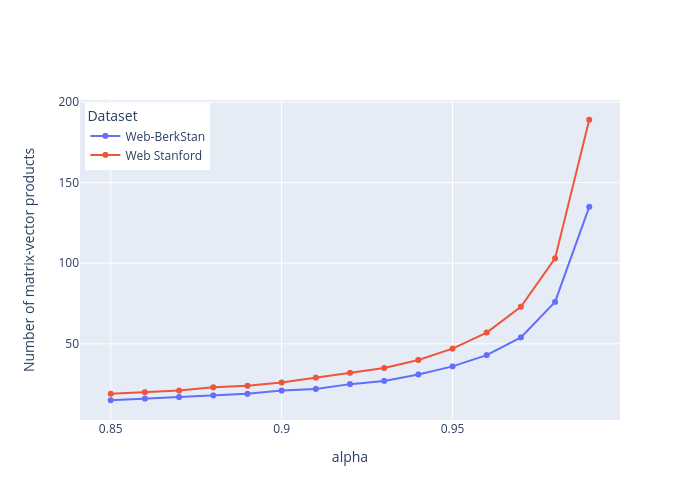
\includegraphics[width=1\textwidth]{mv_alpha.png}
    \caption{Number of matrix-vector products required for the standard Power method for different values of $\alpha$.}
    \label{fig:mv}
\end{figure}


\begin{table}[h]
    \centering
    \begin{tabular}{|c|cc|}
        \hline
        \textbf{} & \multicolumn{1}{c|}{\textbf{Web-Stanford}} & \textbf{Web-BerkStan} \\ \hline
        $\alpha$  & \multicolumn{2}{c|}{\textit{matrix-vector products}}                                   \\ \hline
        $0.85$         & \multicolumn{1}{c|}{19}                     & 15                     \\ \hline
        $0.86$         & \multicolumn{1}{c|}{20}                     & 16                     \\ \hline
        $0.87$         & \multicolumn{1}{c|}{21}                     & 17                     \\ \hline
        $0.88$         & \multicolumn{1}{c|}{23}                     & 18                     \\ \hline
        $0.89$         & \multicolumn{1}{c|}{24}                     & 19                     \\ \hline
    $0.90$         & \multicolumn{1}{c|}{26}                     & 21                     \\ \hline
    $0.91$         & \multicolumn{1}{c|}{29}                     & 22                     \\ \hline
    $0.92$         & \multicolumn{1}{c|}{32}                     & 25                     \\ \hline
    $0.93$         & \multicolumn{1}{c|}{35}                     & 27                     \\ \hline
    $0.94$         & \multicolumn{1}{c|}{40}                     & 31                     \\ \hline
    $0.95$         & \multicolumn{1}{c|}{47}                     & 36                     \\ \hline
    $0.96$         & \multicolumn{1}{c|}{57}                     & 43                     \\ \hline
    $0.97$         & \multicolumn{1}{c|}{73}                     & 54                     \\ \hline
    $0.98$         & \multicolumn{1}{c|}{103}                    & 76                     \\ \hline
    $0.99$         & \multicolumn{1}{c|}{189}                    & 135                    \\ \hline
\end{tabular}
\caption{Table of the results}
\label{tab:mv}
\end{table}

